
\documentclass{article}

%encoding
%--------------------------------------
\usepackage[utf8]{inputenc}
\usepackage[T1]{fontenc}
%--------------------------------------

\usepackage{geometry}
\usepackage{amsmath}
\usepackage{graphicx}
\usepackage{float}

\usepackage[brazilian]{babel}
\usepackage{hyphenat}
\hyphenation{mate-mática recu-perar}

 \geometry{
 a4paper,
 total={170mm,257mm},
 left=20mm,
 top=20mm,
 }

\title{Relatório do trabalho 5}
\date{21/06/2019}
\author{Allan Nozomu Fukasawa RA:163527}

\begin{document}
\maketitle

\section{Introdução}

O objetivo deste trabalho é aplicar técnicas de agrupamentos de dados (técnincas de aprendizago de máquina não supervisionado) para reduzir o número de cores de uma imagem colorida, sempre tentando manter a qualidade original da imagem. Para isso, usaremos uma técnica de agrupamento k-means, a qual explicaremos melhor ainda.

Os passos seguidos para a execução do trabalho foram extraídos de sua especificação. \cite{Helio:1}

\section{Componentes}

Está sendo enviado junto a este relatório os seguintes arquivos e diretórios:

\begin{itemize}
  \item arquivo Trabalho 5.ipynb: contém todo o código executado durante este trabalho.

  \item quatro imagens utilizadas durante o processamento (todas estão disponíveis pelo professor no seguinte link \textit{http:\/\/www.ic.unicamp.br/\~helio\/imagens\_coloridas\/}. No arquivo do Jupyter Notebook, está sendo utilizada a imagem do Baboon (\textit{baboon.png}), disponível na Figura \ref{Fig:original}.

  \item 6 imagens de resultado com diferentes quantidades de cores: 4, 8, 16, 32, 64 e 128. Todas estão disponíveis na pasta \textit{images/res*}.

\end{itemize}

\begin{figure}[!htb]
  \centering
  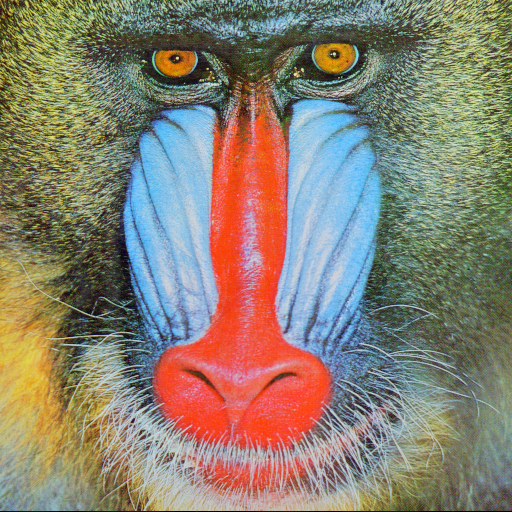
\includegraphics[width=.5\linewidth]{images/baboon.png}
  \caption{Imagem original}\label{Fig:original}
\end{figure}

\subsection{O Programa}

O programa foi implementado com Jupyter Notebooks, usando Python 3.7.1. As bibliotecas utilizadas no desenvolvimento do programa foram, com suas respectivas versões: 

\begin{itemize}
    \item numpy (1.15.4): para manipulação dos vetores.

    \item matplotlib (3.0.2): visualização dos dados, resultados finais e intermediários.

    \item opencv (3.4.2): realização da leitura e escrita das imagens, transformação das cores (de BGR para LAB e vice-versa).
    
    \item sklearn (0.20.1): aplicar técnica de agrupamento utilizando k-means e predições

\end{itemize}

\subsection{Formato das imagens}

As imagens de entrada estão no formato PNG (Portable Network Graphics). As imagens de saída também estão no mesmo formato.

\section{Leitura, escrita e plotagem das imagens}

\subsection{Leitura das imagens}

A imagem de entrada é lida com função \textbf{cv2.imread} que armazena a imagem em um \textbf{numpy.ndarray} de 3 dimensões (MxNx3).

Depois de lida, a imagem foi convertida para o formato de cores LaB. Isso porque nesse formato há uma correspondência mais clara entre a distância euclidiana formada pelas componentes nesse sistema de cores do que na BGR (que é lida pelo opencv, por padrão). Dessa forma, as técnincas de agrupamento acabam trazendo informações mais claras. Para isso, utilizou-se a função \textbf{cv2.cvtColor}.

\subsection{Escrita das imagens}

Também foi feito uma função auxiliar para facilitar na saída das imagens utilizando a função \textbf{cv2.imwrite}. 

\subsection{Plotagem das imagens}

Foi utilizado para visualização dos resultados as funções de plotagem de imagens em \textbf{matplotlib.pyplot}. Para isso, antes a imagem era convertida para o formato de cores RGB porque o \textit{opencv} deixa por padrão, as imagens lidas em formato BGR. Para isso, usou-se a função \textbf{cv2.cvtColor}.

\section{Solução}

\subsection{Técnica K-means}

Foi utilizado a técninca \textit{K-means} para o agrupamento de dados com o entuito de encontrar cores mais representativas. Para isso, uso-se a função \textbf{cluster.KMeans} passando como parâmetro o número de clusters desejados (a quantidade de cores desejadas).

Depois, salvou-se os resultados dos centros dos grupos (centróides), juntamente com os rótulos correspondentes de cada pixel da imagem. Dessa forma, foi possível classificar para cada pixel, qual era a cor que mais se aproximava (em qual cluster esta pertencia).

Também foi medido o tempo de processamento das técnicas de agrupamento para se ter uma ideia da performance e robustez do algoritmo.

\subsection{Resultados}

Foram aplicadas ao todos, 7 diferentes classificações, com os seguintes números de cores: 2, 4, 8, 16, 32, 64 e 128. As imagens resultados estão disponíveis entre as figuras \ref{Fig:res2} a \ref{Fig:res128}

Em relação aos tempos de duração para cada número de cores obtemos, em segundos:

\begin{center}
  \begin{tabular}{ | l | c | c | c | c | c | c | c | }
    \hline
    \textbf{Cores} & 2 & 4 & 8 & 16 & 32 & 64 & 128 \\ \hline
    \textbf{Tempo} & 1.2 & 6.1 & 13.4 & 57.2 & 147.1 & 397.3 & 1145.4  \\
    \hline
  \end{tabular}
\end{center}


\begin{figure}[!htb]
  \begin{minipage}{0.42\textwidth}
    \centering
    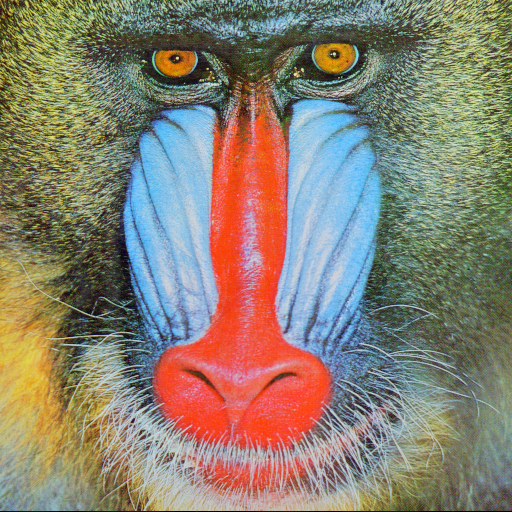
\includegraphics[width=.99\linewidth]{images/baboon.png}
    \caption{Imagem original}\label{Fig:original}
  \end{minipage}\hfill
  \begin{minipage}{0.42\textwidth}
    \centering
    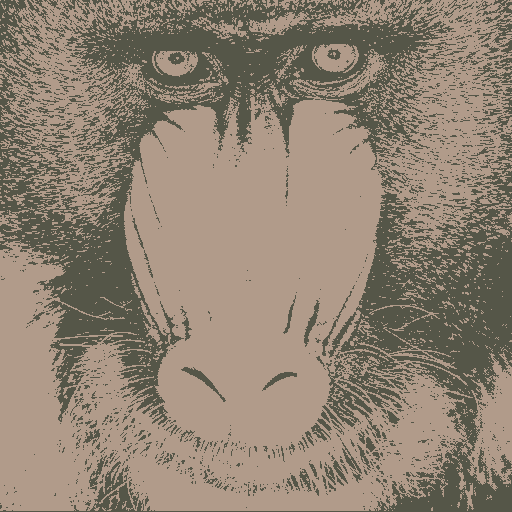
\includegraphics[width=.99\linewidth]{images/res2.png}
    \caption{Resultado com 2 cores}\label{Fig:res2}
  \end{minipage}
\end{figure}

\begin{figure}[!htb]
  \begin{minipage}{0.42\textwidth}
    \centering
    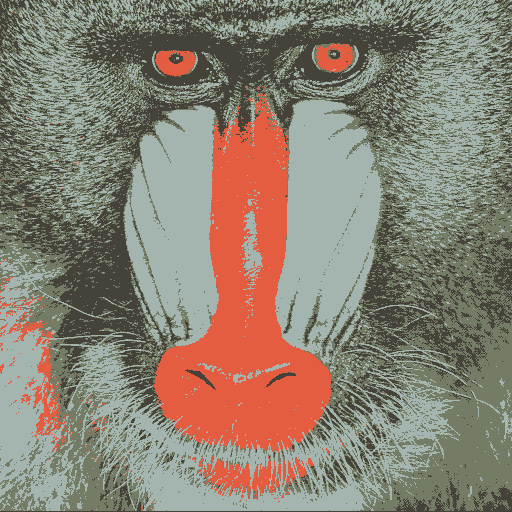
\includegraphics[width=.99\linewidth]{images/res4.png}
    \caption{Resultado com 4 cores}\label{Fig:res4}
  \end{minipage}\hfill
  \begin{minipage}{0.42\textwidth}
    \centering
    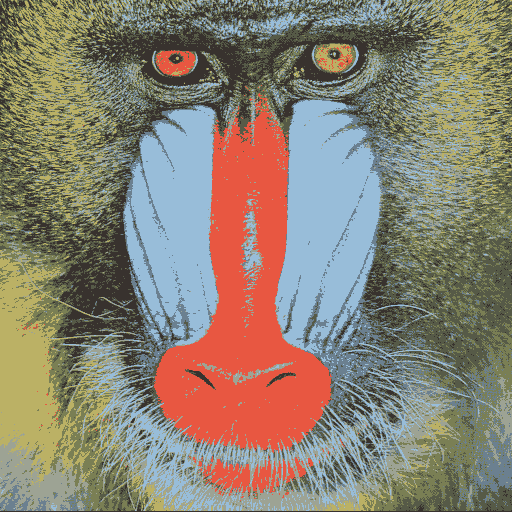
\includegraphics[width=.99\linewidth]{images/res8.png}
    \caption{Resultado com 8 cores}\label{Fig:res8}
  \end{minipage}
\end{figure}

\begin{figure}[!htb]
  \begin{minipage}{0.42\textwidth}
    \centering
    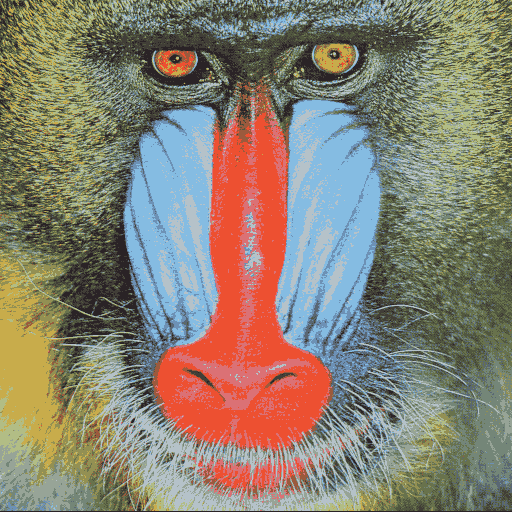
\includegraphics[width=.99\linewidth]{images/res16.png}
    \caption{Resultado com 16 cores}\label{Fig:res16}
  \end{minipage}\hfill
  \begin{minipage}{0.42\textwidth}
    \centering
    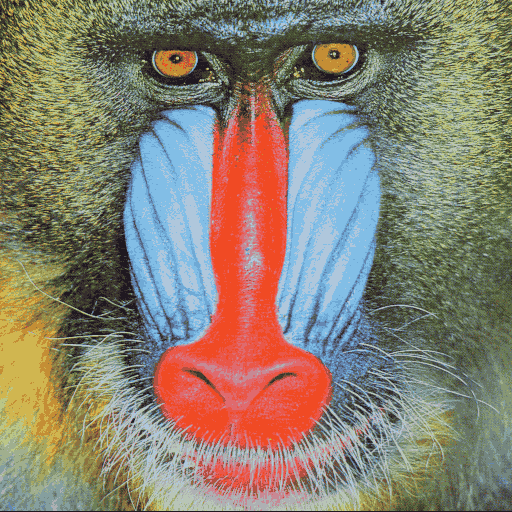
\includegraphics[width=.99\linewidth]{images/res32.png}
    \caption{Resultado com 32 cores}\label{Fig:res32}
  \end{minipage}
\end{figure}

\begin{figure}[!htb]
  \begin{minipage}{0.42\textwidth}
    \centering
    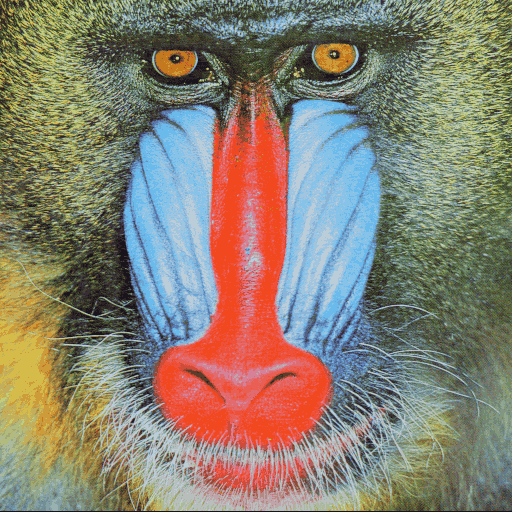
\includegraphics[width=.99\linewidth]{images/res64.png}
    \caption{Resultado com 64 cores}\label{Fig:res64}
  \end{minipage}\hfill
  \begin{minipage}{0.42\textwidth}
    \centering
    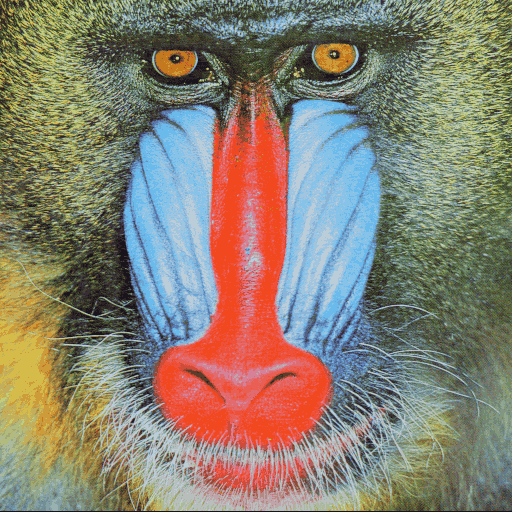
\includegraphics[width=.99\linewidth]{images/res64.png}
    \caption{Resultado com 128 cores}\label{Fig:res128}
  \end{minipage}
\end{figure}


\section{Conclusão}

Após a execução da técnica de agrupamento e analisando os resultados, foi possível quantizar as imagens com as quantidades desejadas.

Analisando os resultados em relação as imagens, podemos notas uma grande diferença de qualidade principalmente em relação às quantidades mais baixas de cores (de 2 a 16 cores). A partir de 32 cores, as diferenças são mínimas, muitas vezes, quase imperceptíveis se comparadas a imagem original. Porém algumas diferenças ainda podem ser notadas principalmente nos pelos e nas cores dos olhos do \textit{baboon}. Isso mostra a qualidade elevada do resultado após a execução do algoritmo.

Porém em relação ao tempo, esta técninca se apresentou muito ineficiente, devido ao método de clusterização do \textit{K-means}. Em números mais baixos, o algortimo apresentou resultados satisfatórios de tempo (com 2 a 8 cores), levando poucos segundos. Porém, com 16 cores, a solução já começou a apresentar problemas de performance, demorando quase 1 minuto. No teste com o maior número de cores (128), levou 1145 segundos (quase 20 minutos de processamento), o que é inviável, ainda mais se tratando de uma imagem relativamente pequena (512x512).

Portanto, a utilização do método \textit{K-means} para quantizar cores de imagens, apesar de ser uma ideia simples e intuitiva, apresenta resultados ineficientes em relação ao tempo de processamento principalemente com um grande números de cores quantizadas. 

\bibliography{relatorio5}
\bibliographystyle{ieeetr}

\end{document}